\chapter{Funktionsreihen}

Eine Funktion ist eindeutig definiert durch ihre Rechenvorschrift, etwa $\sin(x)$ oder $e^x$. Doch wie können wir den Wert eines solchen Ausdrucks für eine konkrete Zahl $x$ berechnen? In der Praxis wird dies in der Regel über Näherungsverfahren getan. Ein solches Näherungsverfahren kann man mithilfe der sogenannte Taylor-Reihe gewinnen, die wir in diesem Kapitel betrachten werden. Die Taylor-Reihe stellt eine spezielle Form einer Funktionsreihe dar. Im ersten Kapitel hatten wir bereits Folgen von Zahlen betrachtet. Analog dazu ist es nun auch möglich, Folgen von Funktionen zu definieren und daraus eine Reihe zu bilden. Doch es gibt auch andere Funktionsreihen, die viele praktische Anwendungen haben. Die sogenannte Fourier-Reihe wird etwa in der Signalanalyse verwendet. Aus einem Audio-Signal, welches aufgenommen wurde als Änderung des Luftdrucks über die Zeit, kann mittels der Fourier-Analyse eine Frequenzspektrum gewonnen werden. Solch ein Frequenzspektrum lässt sich häufig wesentlich besser auf charakteristische Merkmale untersuchen, etwa um in der Spracherkennung herauszufinden, um welches Phonem oder Wort es sich handelt.

\section{Allgemeine Funktionsreihen}

Wir nähern uns dem Begriff der Funktionsreihen, indem wir zuerst endliche Reihen betrachten, also eine Reihe, welche die Summe einer endlichen Anzahl von Funktionen ist. Anschließend überlegen wir uns, was es bedeutet, eine Grenzwertbildung auszuführen. Im Gegensatz zu Zahlenreihen ist hier etwa mehr Vorsicht notwendig, da das Konvergenzverhalten anders sein kann, je nachdem, welches Argument man in die Funktionen einsetzt.

\begin{definition}{Endliche Funktionsreihe}{FunSum}
    Sei $f_n: \R \to \R, n\in\N$  eine Folge von Funktionen, welche alle den Definitionsbereich $\mathbb{D}$ besitzen. Dann versteht man unter der zugehörigen \textbf{endlichen Funktionsreihe} (Partialsummen) $F_n$ die Folge von Funktionen, welche durch Summation der ersten $n+1$-Glieder entsteht:
    $$
        F_n(x) = \sum\limits_{i=0}^n f_(x)
    $$
    Alle Glieder $F_n$ der Funktionsreihe haben den gleichen Definitionsbereich $\mathbb{D}$.
\end{definition}

Für jedes $n$ ist damit eine Funktion definiert, in die wir Argumente aus dem Definitionsbereich einsetzen können und eindeutig einen Funktionswert erhalten. Anders ausgedrückt hängt der Funktionswert also von zwei Variablen ab, dem Index $n$ und dem Argument $x$. Um nun die unendliche Reihe als Grenzwert für große $n$ definieren zu können, müssen wir zuerst den Wert für $x$ festlegen.

\begin{definition}{Grenzfunktion einer Funktionsreihe}{LimFunSum}
    Sei $F_n: \R \to \R$ eine endliche Funktionsreihe mit Definitionsbereich $\mathbb{D}$. Für jedes Argument $x$ ist dann eine Reihe gegeben, welche entweder konvergent ist oder nicht. Die Menge aller Argumente $x$, für welche diese Reihe konvergiert, nennt man das \textbf{Konvergenzintervall} $K$. Die \textbf{Grenzfunktion} ist dann die Abbildung der Argumente aus dem Definitionsbereich zu dem jeweiligen Grenzwert der Funktionsreihe für dieses Argument:
    $$
        F(x) = F_\infty(x) = \lim\limits_{n\to\infty} \sum\limits_{i=0}^n f_i(x)
    $$
\end{definition}

Man beachte dabei, dass zuerst das Argument auf einen festen Wert gesetzt wird und \emph{danach} die Grenzwertbildung ausgeführt wird.

In der praktischen Berechnung wird als Approximation statt der Grenzfunktion manchmal nur die endliche Funktionsreihe verwendet. Dadurch entsteht ein Fehler, der geringer wird, je mehr Glieder der Funktionsreihe man verwendet:

\begin{definition}{Restglied}{ErrorTerm}
    Die Differenz zwischen der Grenzfunktion $F$ und der der endlichen Funktionsreihe $F_n$ im Konvergenzintervall nennt man das Restglied $R_n$.
    $$
        R_n(x) = F(x) - F_n(x) = F(x) - \sum\limits_{i=0}^n f_(x)
    $$
    Im Grenzwert verschwindet das Restglied für alle Argumente aus dem Konvergenzintervall $\mathbb{K}$:
    $$
        \lim\limits_{n\to\infty}(x) = 0 \forall x \in \mathbb{K}
    $$
\end{definition}

Ein Beispiel für eine solche Funktionsreihe haben wir bereits im Kapitel zu Funktionen anhand der \emph{Blancmange-Funktion} gesehen. Diese stellte eine Beispiel für eine stetige, aber nirgends differenzierbare Funktion dar und ist in Abbildung \ref{fig:BlancmangeFunction} dargestellt.

\begin{example}{Funktionsreihe und Grenzfunktion}{FunSumAndLim}
    Durch $fn(x) = x^2 (1-x^2)^n$ ist für jedes $n=0,1,2,\dots$ eine Funktion im Intervall $[-1,1]$ gegeben. Durch Summation erhalten wir die Partialsummen $F_n(x) = \sum\limits_{i=0}^n x^2 (1-x^2)^i$. Die ersten Glieder lauten demnach
    \begin{alignat*}{1}
        F_0(x) &= x^2 \\
        F_1(x) &= x^2 + x^2 (1-x^2) = x^2 (2-x^2) \\
        F_2(x) &= x^2 (2-x^2) + x^2 (1-x^2)^2 = x^2 (x^4-3x^2+3)
    \end{alignat*}
    Um nun die Grenzfunktion zu erhalten, müssen wir für einen festen Wert $x$ den Grenzübergang $n \to \infty$ durchführen. Wenn wir den Funktionsterm $F_n$ genauer anschauen, stellen wir fest, dass es sich für ein festes $x$ um eine geometrische Reihe mit $p=x^2$ und $q=(1-x^2)$ handelt. Wir wissen, dass diese für $|q|=|1-x^2|<1$ konvergiert, also für $x \in [-1,1]$. Für $x=0$ ergibt sich $q=1$, doch da dann auch $p=0$ ist, konvergiert die Reihe für $x=0$ ebenfalls. Somit lautet der Konvergenzbereich der Funktionsreihe $\mathbb{K} = [-1,1]$ und der Grenzwert ergibt sich zu:
    $$
        \lim\limits_{n\to\infty} \sum\limits_{i=0}^n x^2 (1-x^2)^i = \frac{p}{1-q} = \frac{x^2}{1-(1-x^2)} = 1
    $$
    Der Graph für einige Glieder dieser Funktionsreihe findet sich in Abbildung \ref{fig:ExFunSum}. Das Restglied ist ein Maß dafür, wie nah die Partialsummen $F_n$ an der Grenzfunktion $F(x) = 1$ liegen, dies ist in Abbildung \ref{fig:ExFunErrTerm} illustriert.
\end{example}

\begin{figure}
    \centering
    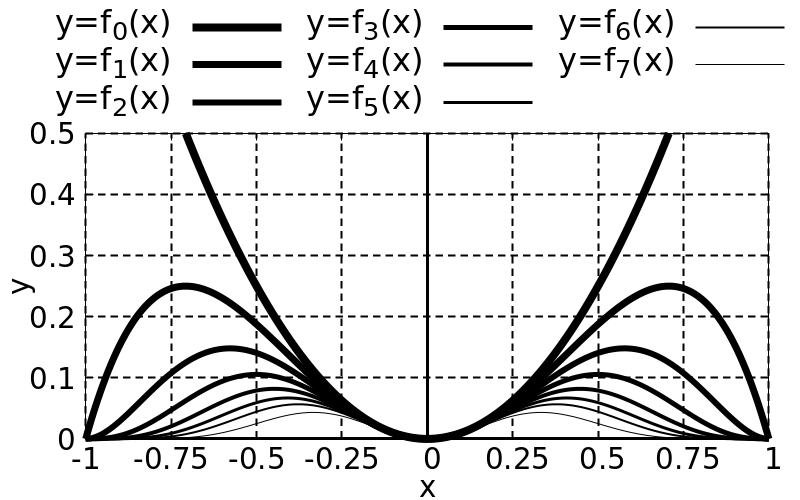
\includegraphics[width=0.45\textwidth]{./gnuplot/example-function-sum}
    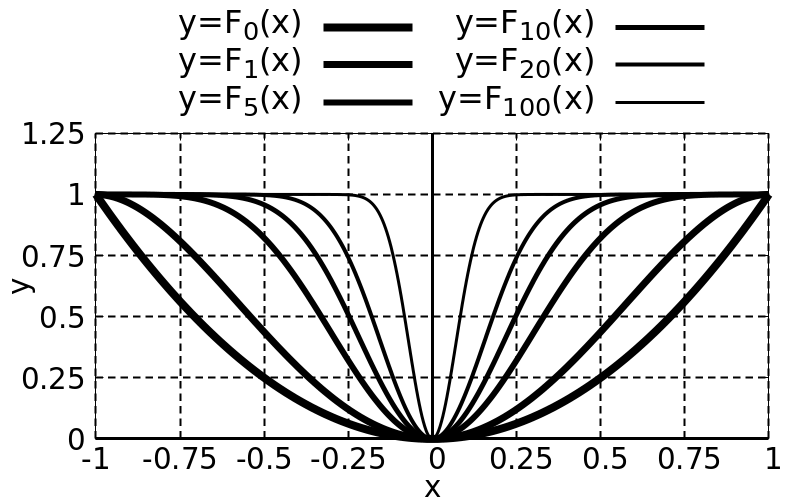
\includegraphics[width=0.45\textwidth]{./gnuplot/example-function-sum-summed}
    \caption[Einzelfunktionen und Partialsummen einer Funktionsreihe]{Beispiel einer Funktionsreihe. Links: Die Einzelfunktion $f_n$. Rechts: Die Partialsummen $F_n$.}
    \label{fig:ExFunSum}
\end{figure}

\begin{figure}
    \centering
    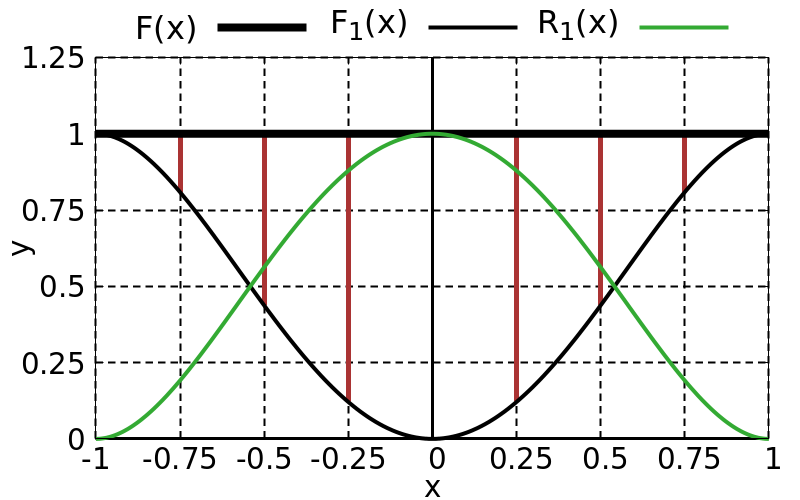
\includegraphics[width=0.65\textwidth]{./gnuplot/function-sum-error-term}
    \caption[Restglied zwischen Grenzfunktion und Partialsumme]{Graphische Bedeutung des Restglied $R_n$ als Differenz (rot) zwischen Grenzfunktion und Partialsumme.}
    \label{fig:ExFunErrTerm}
\end{figure}

Bisher haben wir nur den Grenzwert der Partialsummen für ein gegebenes $x$ betrachtet. Das Konvergenzintervall ist die Menge von Argumenten, wo dieser Grenzwert existiert. Diese Art der Konvergenz nennt man die sogenannte \textbf{punktweise Konvergenz}, da immer nur ein konkretes $x$ betrachtet wird. Jetzt kann es aber sein, dass die Partialsummen für ein bestimmtes $x$ sich dem Grenzwert nur sehr langsam nähern und für ein anderes $x$ sich sehr schnell nähern. Für viele Schlussfolgerungen im Zusammenhang mit Funktionsreihen benötigt man noch eine stärkere Art der Konvergenz. Man fordert, dass die Partialsummen für alle Argument gleich schnell, also \emph{gleichmäßig}, gegen ihren Grenzwert laufen.

\begin{definition}{Gleichmäßige Konvergenz einer Funktionsreihe}{UniformConv}
    Eine Funktionsreihe $F_n$ heißt auf einem Konvergenzintervall $\mathbb{K}$ \textbf{gleichmäßig konvergent} gegen die Grenzfunktion $F$, wenn in der Epsilon-Definition des Grenzwerts (siehe \ref{def:Convergence}) das erste Folgenglied, ab dem alle weiteren Folgenglieder einen Abstand von weniger als Epsilon vom Grenzwert haben, nur von dem gewählten Epsilon, aber nicht vom konkreten Argument $x\in\mathbb{K}$ abhängt.
    $$
        \forall \epsilon > 0 \exists n_0: \forall n > n_0, x \in \mathbb{K}: |F-F_n(x)| = |R_n(x)| < \epsilon
    $$
\end{definition}

Manchmal ist es einfacher, eine Funktion als Grenzfunktion einer Funktionsreihe darzustellen. Wie können wir von der Grenzfunktion Ableitung und Integral berechnen? Naiv könnte man jetzt auf die Idee kommen, einfach die Summanden der Funktionsreihe separat abzuleiten oder zu integrieren. Es zeigt sich aber, dass dies im allgemeinen aufgrund der Grenzwertbildung nicht möglich ist. Für gleichmäßig konvergente Funktionsreihen gilt aber die folgende Aussage:

\begin{statement}{Gliedweise Differenzierbarkeit und Integrierbarkeit}{DiffIntByParts}
    Eine auf einem Konvergenzintervall $\mathbb{K}$ gegen eine Grenzfunktion $F$ gleichmäßig konvergente Funktionsreihe $F_n$ kann gliedweise differenziert und integriert werden.
    \begin{alignat*}{1}
        \dd{}{x} F(x)      &= \lim\limits_{n\to\infty} \sum\limits_{i=0}^n \dd{}{x} f_i(x) \\
        \int F(x) \diff{x} &= \lim\limits_{n\to\infty} \sum\limits_{i=0}^n \int f_i(x) \diff{x}
    \end{alignat*}
\end{statement}

\begin{example}{Gliedweise Ableitung einer nicht gleichmäßig konvergenten Funktionsreihe}{ExNonUniformFunSum}
    Die Grenzfunktion $\sum\limits_{n=1}^\infty \frac{\sin(nx)}{n}$ existiert für alle reellen Argument $x$, beispielsweise ist $\sum\limits_{n=1}^\infty \frac{\sin(n)}{n} = \frac{\pi-1}{2}$. Leitet man nun aber jedes Glied ab, erhält man $\sum\limits_{n=1}^\infty \cos(nx)$. Diese Reihe divergiert für jedes $x$. Dies liegt daran, dass die Funktionsreihe zwar punktweise konvergent, aber nicht gleichmäßig konvergent ist.
\end{example}

\section{Potenzreihen}

Potenzreihen sind eine besondere Form von Funktionsreihen, bei denen jede Funktion $f_n$ eine Polynom vom Grad $n$ ist. Die Funktionsreihe ist damit eindeutig gegeben durch Angabe der Koeffizienten $a_n$ vor den jeweiligen Monomen. Beispielsweise ist $1+x+x^2/2+x^3/6+x^4/24 + \dots + x^n/n! + \dots$ eine solche Potenzreihe.

\begin{definition}{Potenzreihe}{PowerSum}
    Unter einer \textbf{Potenzreihe} versteht man eine Funktionsreihe, die aus Polynomen mit Koeffizienten $a_i$ gebildet wird:
    \begin{alignat*}{1}
        F_n(x) &= \sum\limits_{i=0}^n a_i x^i \\
        F(x)   &= \sum\limits_{n=0}^\infty a_n x^n
    \end{alignat*}
\end{definition}

Wir können uns nun die Frage stellen, für welche $x$ eine solchen Potenzreihe konvergiert. Offensichtlich liegt für $x=0$ Konvergenz vor, da dann alle Summanden bis auf das konstante Glied identisch $0$ sind. Um herauszufinden, für welche $x$ noch Konvergenz vorliegt, betrachten wir $x$ als Konstanten und wenden wir das Wurzelkriterium \ref{stmt:RootTest} für Reihen an. Die einzelnen Folgenglieder lauten dann $b_n = a_n \cdot x^n$.

\begin{alignat*}{1}
    q &= \lim\limits_{n\to\infty} \nroot{n}{|b_n|} \\
      &= \lim\limits_{n\to\infty} \nroot{n}{|a_n x^n|} \\
      &= \lim\limits_{n\to\infty} \nroot{n}{|a_n| \cdot |x|^n} \\
      &= \lim\limits_{n\to\infty} \nroot{n}{|a_n|} |x| \\
      &= |x| \cdot \lim\limits_{n\to\infty} \nroot{n}{|a_n|}
\end{alignat*}

Nach dem Wurzelkriterium muss nun $q<1$ gelten, damit die Reihe konvergent ist:

\begin{alignat*}{1}
             & |x| \cdot \lim\limits_{n\to\infty} \nroot{n}{|a_n|} < 1 \\
    \implies & |x| < \underbrace{\frac{1}{\lim\limits_{n\to\infty} \nroot{n}{|a_n|}}}_R
\end{alignat*}

Damit haben wir herausgefunden, dass die Potenzreihe dann konvergent ist, wenn das Argument betragsmäßig kleiner ist als der Grenzwert $R$ auf der rechten Seite. Anders ausgedrückt muss das Argument im offenen Intervall $(-R,R)$ liegen. Außerhalb dieses Intervalls, für $x > R$ beziehungsweise $x<-R$ ist $q>1$ und nach dem Wurzelkriterium die Reihe damit divergent. Am Rand dieses Intervalls ($-R,R$) ist $q=1$ und das Wurzelkriterium liefert keine Aussage, hier ist eine separate Betrachtung notwendig. Der Wert von $R$ hängt nur von den Koeffizienten $a_n$ ab und kann berechnet werden.

Die gleiche Betrachtung kann man jetzt noch einmal mit dem Quotientenkriterium \ref{stmt:RatioTest} durchführen. Wir erhalten damit die folgende Aussage.

\begin{statement}{Konvergenzradius einer Potenzreihe}
    Eine Potenzreihe $F_n(x) = \sum\limits_{i=0}^n a_i x^i$ ist für alle Argumente $|x| < R$ innerhalb des \textbf{Konvergenzradius} $R$ gleichmäßig konvergent. Der Konvergenzradius kann berechnet werden zu:
    \begin{alignat*}{1}
        1/R &= \lim\limits_{n\to\infty} \nroot{n}{|a_n|} \\
            &= \lim\limits_{n\to\infty} |\frac{a_{n+1}}{a_n}|
    \end{alignat*}
    Für $1/R=0$ ist dabei der Konvergenzradius $\infty$, die Potenzreihe konvergiert also für alle reellen Zahlen. Für $1/R=\infty$ konvergiert die Potenzreihe nirgends (bis auf $x=0$).
\end{statement}

Da die Potenzreihe im Konvergenzradius gleichmäßig konvergent ist, kann sie also gliedweise differenziert und integriert werden.

\begin{example}{Berechnung des Konvergenzradius}{ExCompConvRad}
    Wir betrachten die Potenzreihe $F_n(x) = \sum\limits_{i=0}^n \frac{1}{i!} x^i$. Die Folge der Koeffizienten lautet $a_n=\frac{1}{n!}$. Der Konvergenzradius berechnet sich über das Quotientenkriterium zu
    \begin{alignat*}{1}
        1/R &= \lim\limits_{n\to\infty} \frac{a_{n+1}}{a_n} \\
            &= \lim\limits_{n\to\infty} \frac{n!}{(n+1)!} \\
            &= \lim\limits_{n\to\infty} \frac{1}{n+1} \\
            &= 0
    \end{alignat*}
    Damit lautet der Konvergenzradius $\infty$, die Potenzreihe konvergiert also für alle reellen Argumente $x$.
\end{example}


\section{Taylor-Entwicklung}

Die Taylor-Entwicklung ist eine Rechenmethode, mit der man für eine gegebene Funktion $f$ eine Potenzreihe berechnen kann, deren Grenzfunktion der Funktion $f$ entspricht. Allerdings ist dies nicht für alle Funktionen möglich. Zur Herleitung der Taylor-Formel nehmen wir an, eine Funktion $f$ sei in eine Potenzreihe entwickelbar:

$$
    f(x) = a_0 + a_1 x + a_2 x^2 + a_3 x^3 + \dots
$$

Wie können wir dann die Koeffizienten $a_n$ bestimmen? Falls die linke und rechte Seite in der obigen Gleichung für alle Argumente $x$ im Konvergenzbereich der Potenzreihe gelten soll, muss sie speziell auch für $x=0$ gelten, dass immer zum Konvergenzradius gehört. Setzen wir $x=0$, ergibt sich:

$$
    f(0) = a_0
$$

Somit haben wir den ersten Koeffizienten $a_0 = f(0)$ der Potenzreihe bestimmt. Um den nächsten Koeffizienten zu bestimmten, leiten wir beide Seiten einmal nach $x$ ab und setzen wieder $x=0$:

\begin{alignat*}{1}
    f'(x) &= a_1 + 2 a_2 x + 3 a_3 x^2 + \dots \\
    f'(0) &= a_1
\end{alignat*}

Also lautet der zweite Koeffizient $a_1 = f'(0)$ Durch erneutes Ableiten ergeben schrittweise die weiteren Koeffizienten:

\begin{alignat*}{1}
    f''(x)  &= 2 a_2 + 6 a_3 x + \dots \\
    f'''(x) &= 6 a_3 + \dots \\
    f''(0)  &= 2 a_2 \\
    f'''(0) &= 6 a_3
\end{alignat*}

Spätestens erkennen wir ein Muster. Der Koeffizient $a_n$ ergibt sich immer als Wert der $n$-ten Ableitung von $f$ an der Stelle $0$, geteilt durch $n!$ (welches sich durch $n$-faches Ableiten des Monoms $x^n$ ergibt).

Nun sind wir bisher immer von einer Potenzreihe ausgegangen, welche um die Stelle $0$ zentriert war. Aus dem vorigen Abschnitt zu Funktionen wissen wir aber, dass wir Funktionen entlang der x-Achse um $x_0$ verschieben können, in wir das Argument durch $x \to x-x_0$ ersetzen. Damit ergibt sich die allgemeine Form der Taylor-Entwicklung:

\begin{definition}{Taylor-Reihe}{TaylorExpansion}
    Die durch eine Funktion $f$ an der \textbf{Entwicklungsstelle} $x_0$ erzeugte \textbf{Taylor-Reihe} vom \textbf{Grad n} ist gegeben durch:
    $$
        f(x) = \underbrace{\sum\limits_{i=0}^n \frac{f^{(n)}(x_0)}{n!} (x-x_0)^n}_{\text{Taylor-Reihe}} + \underbrace{R_n(x)}_{\text{Restglied}}
    $$
    Konvergiert das Restglied gegen $0$, dann hat die Taylor-Reihe $f$ als Grenzfunktion. Man sagt dann, die Funktion $f$ sei in eine Taylor-Reihe oder Potenzreihe entwickelbar.
\end{definition}

Graphisch betrachtet kann man sich die Taylor-Reihe vom Grad $n$ vorstellen als das Polynom $p_n$ vom Grad $n$, welches sich an der Stelle $x_0$ am besten an die Funktion anschmiegt. Dies ist in Abbildung \ref{fig:GraphTaylor} abgebildet. Das Polynom ist dann eine Näherung der Funktion $f$, die umso besser ist, je näher man an der Stelle $x_0$ ist. Zudem lässt sich die Näherung durch Erhöhung von $n$ verbessern. Tatsächlich ist die Taylor-Entwicklung ein Spezialfall der linearen Näherung einer Funktion für eine Tangente, denn die Taylor-Reihe vom Grad $1$ lautet

$$
    f(x) \approx f(x_0) + f'(x_0) (x-x_0)
$$

Das ist genau die Formel für die Tangente an die Funktion $f$ im Punkt $x_0$.

\begin{figure}
    \centering
    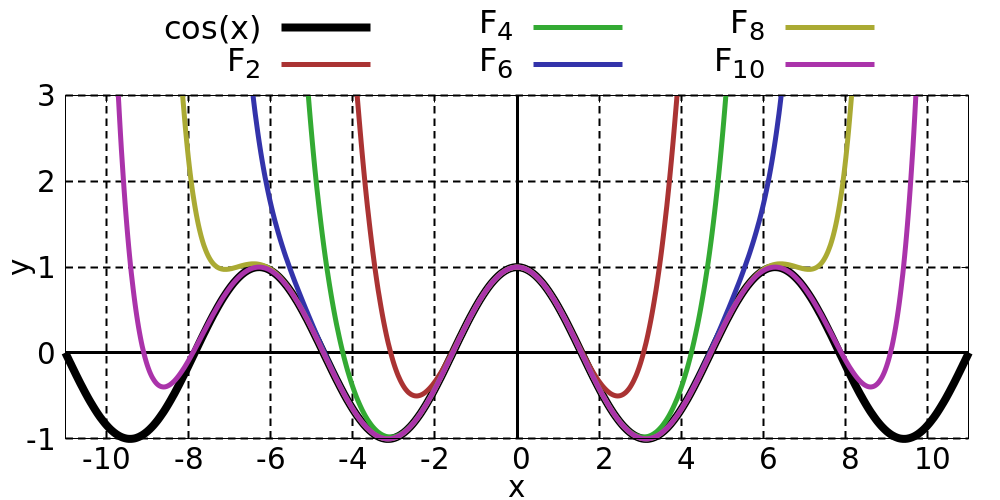
\includegraphics[width=0.65\textwidth]{./gnuplot/taylor-approximation}
    \caption[Approximation einer Funktion mittels Taylorentwicklung]{Graphische Bedeutung des der Taylorentwicklung als Approximation einer Funktion (hier: $\cos(x)$) mittels Polynomen, welche sich an der Entwicklungsstelle an die Funktion anschmiegen.}
    \label{fig:GraphTaylor}
\end{figure}

\begin{example}{Taylor-Reihe konvergiert nicht gegen Grenzfunktion}
    Wir betrachten die Taylor-Reihe, welche durch die Funktion $f(x) = e^{-\frac{1}{x^2}}$ (genauer: ihre stetige Ergänzung) an der Entwicklungsstelle $x_0=0$ erzeugt wird. Alle Ableitungen von $f$ sind von der Form $e^{-\frac{1}{x^2}} \cdot \frac{p(x)}{q(x)}$, wobei der letztere Teil eine gebrochenrationale Funktion ist. An der Entwicklungsstelle $x\to 0$ muss der Wert der $n$-ten Ableitung durch Grenzwertbildung berechnet werden. Durch mehrfache Anwendung der Regel von L'Hôpital lässt sich zeigen, dass die Exponentialfunktion im Grenzwertprozess $x\to 0$ dominiert. Damit sind alle Ableitungen an der Stelle $x_0=0$ identisch $0$. Die Taylor-Reihe lautet mithin $F_n(x) = 0$. Sie ist konvergent und hat die Grenzfunktion $F(x) = 0$. Wir haben hier ein Beispiel gefunden, wo die Taylor-Reihe existiert und konvergent ist, aber eben nicht gegen die Ausgangsfunktion $e^{-\frac{1}{x^2}}$ konvergiert.
\end{example}

\begin{example}{Berechnung der Taylor-Reihe}{CompTaylExp}
    \begin{enumerate}
        \item Alle Ableitungen von $f(x)=e^x$ sind $e^x$. An der Entwicklungsstelle $x_0=0$ ist $e^0 = 1$. Damit ist die Taylor-Reihe der Exponentialfunktion
        \begin{equation}
            e^x = 1 + x + \frac{1}{2} x^2 + \frac{1}{6}x^3 + \dots = \sum\limits_{n=0}^\infty \frac{x^n}{n!}
        \end{equation}
        Der Konvergenzradius dieser Potenzreihe ist $\infty$, wie wir bereits im Beispiel \ref{ex:ExCompConvRad} gesehen haben.
        \item Die Ableitungen von $f(x) =\sin(x)$ sind abwechselnd Sinus- und Kosinusfunktionen. Alle geraden Ableitungen sind Sinusfunktionen und daher bei $x_0=0$ identisch $0$. Für die ungeraden Ableitungen gilt $f'(x) = \cos(x)$, $f'''(x) = -\cos(x)$ und so fort. Ihre Taylor-Reihe ist damit ähnlich zu der für die Exponentialfunktion, mit dem Unterschied dass sie nur ungerade Potenzen enthält (da die Sinusfunktion eine ungerade Funktion ist) und sich die Vorzeichen abwechseln.
        \begin{equation}
            \sin(x) = x - \frac{1}{3!}x^3 + \frac{1}{5!} x^5 \mp \dots
        \end{equation}
        Diese Taylor-Reihe kann man etwa benutzen, um Wert der Sinusfunktion mit beliebiger Genauigkeit zu berechnen.
        \item Analog gilt für die Kosinusfunktion:
        \begin{equation}
            \cos(x) = 1 - \frac{1}{2}x^2 + \frac{1}{4!} x^4 \pm \dots
        \end{equation}
    \end{enumerate}
\end{example}

\begin{example}{Taylor-Reihe mit endlichen Konvergenzradius}{CompTaylorLn}
    Wir wollen die durch $f(x) = \ln(1+x)$ an der Entwicklungsstelle $x_0$ erzeugte Taylor-Reihe ermitteln. Dazu benötigen wir zuerst die Ableitungen:
    \begin{alignat*}{1}
    f^{(1)}(x) &= (1+x)^{-1} \\
    f^{(2)}(x) &= (-1) (1+x)^{-2} \\
    f^{(3)}(x) &= (-1)(-2) (1+x)^{-3} \\
    f^{(4)}(x) &= (-1)(-2)(-3) (1+x)^{-4}
    \end{alignat*}
    Allgemein gilt also $f^{(n)}(x) = (-1)^{n+1} (n-1)! (1+x)^{-n}$. Für $x_0=0$ folgt damit $f^{(n)}(0) = (-1)^{n+1} (n-1)!$ Damit erhalten wir für die Taylorreihe
    $$
        F(x) = \sum\limits_{n=0}^\infty \frac{1}{n!} (n-1)! (-1)^{n+1} x^n = \sum\limits_{n=0}^\infty \underbrace{\frac{(-1)^{n+1}}{n}}_{=a_n} x^n
    $$
    Für den Konvergenzradius dieser Potenzreihe wenden wir das Wurzelkriterium auf die Koeffizienten $a_n$ an:
    $$
        1/R = \lim\limits_{n\to\infty} \nroot{n}{|a_n|} = \lim\limits_{n\to\infty} \nroot{n}{\frac{1}{n}} = \lim\limits_{n\to\infty} 1 / \nroot{n}{n} = 1
    $$
    Der Konvergenzradius beträgt also nur $1$, die Potenzreihe konvergiert nur im Intervall $(-1,1)$ Rechts von der Stelle $x=1$ schnellt die Taylor-Reihe von der Funktion $f$ weg, unabhängig davon, wie viele Glieder man einbezieht. Dieses Verhalten ist in Abbildung \ref{fig:ExTaylorLog} dargestellt.
\end{example}

\begin{figure}
    \centering
    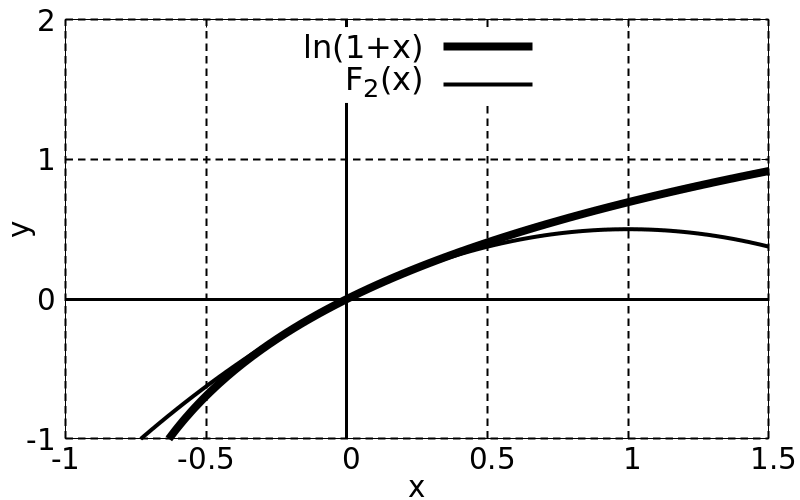
\includegraphics[width=0.45\textwidth]{./gnuplot/taylor-expansion-log-1}
    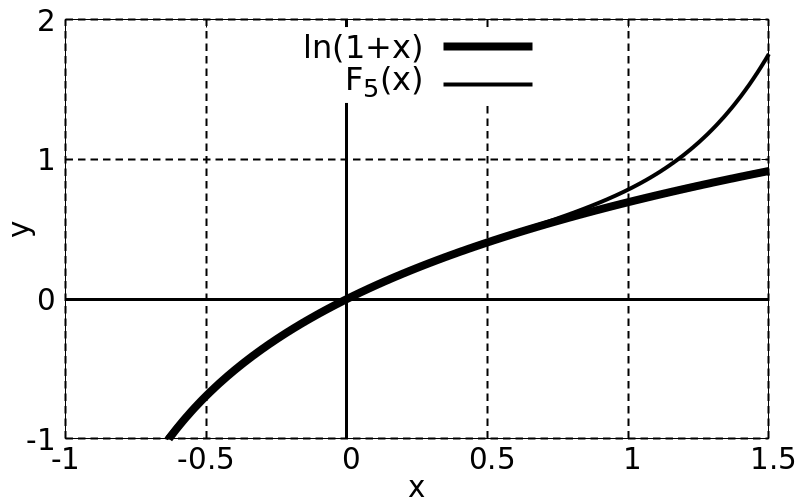
\includegraphics[width=0.45\textwidth]{./gnuplot/taylor-expansion-log-2}
    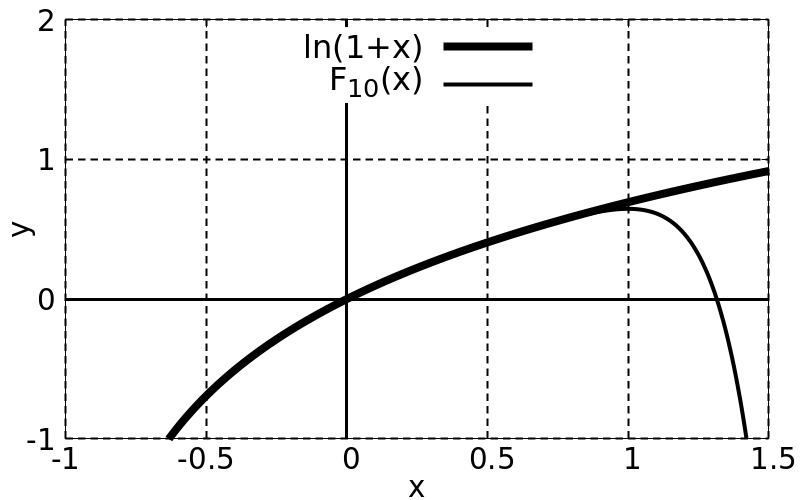
\includegraphics[width=0.45\textwidth]{./gnuplot/taylor-expansion-log-3}
    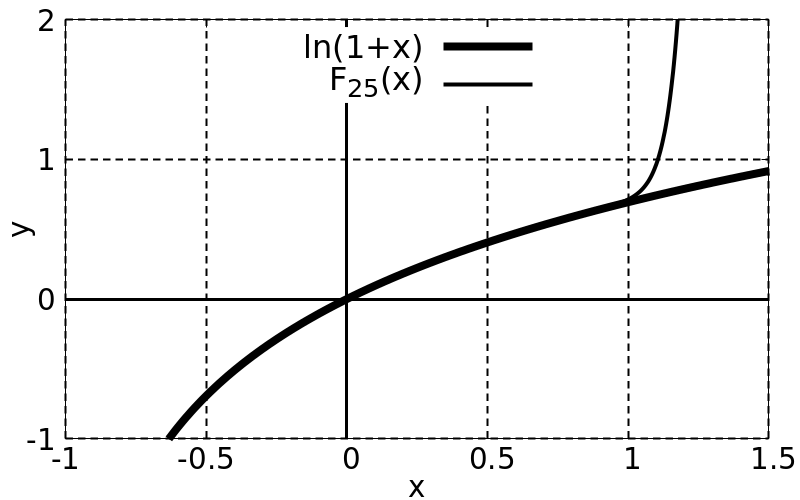
\includegraphics[width=0.45\textwidth]{./gnuplot/taylor-expansion-log-4}
    \caption[Partialsummen von Taylorreihen]{Taylor-Reihen $F_n$ der Funktion $\ln(1+x)$ für verschiedene $n$. Man erkennt, dass für $x>1$ die Reihe nicht mehr konvergiert.}
    \label{fig:ExTaylorLog}
\end{figure}

Um zu zeigen, dass eine Funktion in eine Potenzreihe entwickelbar ist, reicht es nicht aus, nur die Taylor-Reihe aufzustellen. Wir müssen zum einen zeigen, welchen Konvergenzradius die entstehende Potenzreihe hat. Doch es reicht nicht aus, dass die Potenzreihe nur konvergiert, zusätzlich müssen wir zeigen, dass die Grenzfunktion auch die Funktion $f$ ist. Dazu haben wir nachzuweisen, dass das Restglied $R_n$ für große $n$ verschwindet. Doch wie können wir das Restglied berechnen, ohne von der Grenzfunktion Gebrauch zu machen? Darüber gibt der folgende Satz Auskunft:

\begin{statement}{Restgliedform nach Lagrange}{TaylorErrPartLagrange}
    Das Restglied $R_n$ einer durch eine Funktion $f$ um die Stelle $x_0$ erzeugte Taylor-Reihe vom Grad $n$ kann dargestellt werden als:
    $$
        R_n(x) = \frac{(x-x_0)^{n+1}}{(n+1)!} f^{(n+1)}(\vartheta)
    $$
    Dabei ist $\vartheta$ eine Zahl zwischen (inklusive) der Entwicklungsstelle und dem Argument $x$.
\end{statement}

Nun macht diese Restgliedform keine Aussage darüber, welches $\vartheta$ wir denn nun nehmen sollen. Die Aussage ist lediglich, dass es ein $\vartheta$ zwischen der Entwicklungsstelle und dem Argument $x$ gibt, für die die Gleichung für das Restglied korrekt ist. $\vartheta$ hängt dabei aber in der Regel von $x$ ab. Auch wenn wir $\vartheta$ nicht genau bestimmen können, hilft diese Restgliedform dabei. Wir können zumindestens versuchen, eine Abschätzung für das Restglied zu ermitteln, um den maximalen Fehler bei einer Taylor-Reihe vom Grad $n$ zu erhalten.

Dazu betrachten wir den Betrag $|R_n|$ des Restglieds. Wir wählen $\vartheta$ im erlaubten Intervall so, dass der Wert von $f^{(n+1)}(\vartheta)$ maximal wird. Damit erhalten wir die folgende Abschätzung:

\begin{statement}{Restgliedabschätzung}{ErrTermApprox}
    Für das Restglied $R_n$ einer Taylor-Reihe vom Grad $n$ einer Funktion $f$ um die Stelle $x_0$ gilt die folgende \textbf{Restgliedabschätzung}:
    $$
        |R_n(x)| \le \frac{|x-x_0|^{n+1}}{(n+1)!} \max\limits_{\vartheta \in [x,x_0]} f^{(n+1)}(\vartheta)
    $$
\end{statement}

Die Schreibweise $\max\limits{\dots} f$ meint dabei das Maximum von $f$ innerhalb der gegebenen Grenzen des Arguments. Die Schreibweise $[x, x_0]$ meint dabei immer die Zahlen zwischen $x$ und $x_0$. Falls etwa $x=3, x_0=2$, ist mit $[3,2]$ das Intervall $[2,3]$ gemeint.

Schafft man es nun zu zeigen, dass diese Restgliedabschätzung im Grenzwert verschwindet, so tut es auch das Restglied. Ein andere Anwendungsfall ist die Fehlerabschätzung, wenn man eine Funktion durch endliche viele Glieder der Taylor-Reihe nähert.

\begin{example}{Grenzfunktion der Taylor-Reihe der Exponentialfunktion}{LimTaylorExp}
    Die durch die Exponentialfunktion erzeugte Taylor-Reihe ist überall konvergent und lautet $F_n(x) = \sum\limits_{i=0}^n \frac{x^i}{i!} + R_n(x)$. Für das Restglied gilt nach der Abschätzung:
    $$
        |R_n(x)| \le  \frac{|x|^{n+1}}{(n+1)!} \underbrace{\max\limits_{|\vartheta| < x} e^(\vartheta)}_{=e^x}
    $$
    Nach Formel \ref{eq:LimitPowerFactorial} gilt $\lim\limits_{n\to\infty} \frac{a^n}{n!} = 0$ für alle $a$, daher folgt für das Restglied $\lim\limits_{n\to\infty} R_n(x) = $. Somit konvergent die Taylor-Reihe überall gegen die Grenzfunktion $e^x$.
\end{example}

\begin{example}{Fehlerabschätzung mittels Restglied}{ErrTermApprox}
    Wir wollen den Wert $\cos(\degrees{89})$ näherungsweise bestimmen. Dazu entwickeln wir $f(x) = \cos(x)$ um die Entwicklungsstelle $\degrees{90}$ in eine Taylor-Reihe vom Grad $1$. Für die Ableitungen gilt $f'(x) = -\sin(x)$, $f''(x) = -\cos(x)$, $f'''(x) = -\sin(x)$. An der Entwicklungsstelle lauten damit die Werte $f(\degrees{90}) = 0$, $f'(\degrees{90}) = -1$, $f''(\degrees{90}) = 0$, $f'''(\degrees{90}) = 1$. Die Taylor-Reihe vom Grad $1$ ergibt sich zu:
    \begin{alignat*}{1}
        \cos(x) &= f(\degrees{90}) + f'(\degrees{90}) (x-\degrees{90}) + R_1(x) \\
                &= -(x-\degrees{90}) + R_1(x)
    \end{alignat*}
    Für $\cos(\degrees{89})$ erhalten wir so als Näherung $-\degrees{1} = \frac{\pi}{180} \approx \num{0.0174532925}\dots$. Um den Fehler zum wahren Wert von $\cos(\degrees{89})$ abzuschätzen, benutzen wir die Restgliedabschätzung. Da die zweite Ableitung an der Entwicklungsstelle $0$ ist, ist die Taylor-Reihe vom Grad $1$ mit der vom Grad $2$ identisch, wir können also statt $R_1$ auch $R_2$ verwenden. Dazu benötigen wir das Maximum von $f'''(x) = \sin(x)$ im Intervall $[\degrees{89}, \degrees{90}]$. Da die Sinusfunktion zwischen $\degrees{0}$ und $\degrees{90}$ monoton steigend ist, beträgt der Maximalwert $\sin(\degrees{90}) = 1$. Nun erhalten wir als Abschätzung für das Restglied:
    \begin{alignat*}{1}
        |R_2(\degrees{89})| &\le \frac{|-\degrees{1}|^3}{3!} \cdot 1 \\
                           &= \frac{\pi^3}{180^3 \cdot 6} \approx \num{0.000001}
    \end{alignat*}
    Wir können daher aussagen, dass unsere Schätzung bis auf die fünfte Kommastelle genau ist: $\cos(\degrees{89}) \approx  \num{0.017453} \pm \num{0.000001}$. Tatsächlich ist $\cos(\degrees{89}) = \num{0.017452406}\dots$
\end{example}

\begin{definition}{Analytische Funktion}{AnalFun}
    Eine Funktion, die im gesamten Definitionsbereich als Taylor-Reihe dargestellt werden kann, heißt \textbf{analytische Funktion}.
\end{definition}

Bemerkenswert an der Taylor-Entwicklung ist, dass diese nur von dem Wert der Funktion und ihren Ableitung an der Entwicklungsstelle abhängt. Nur Werte nahe der Entwickklungsstelle spielen eine Rolle, da diese für die Ableitung (Grenzwert des Differenzenquotienten) bedeutsam sind. Werte "weit weg" von der Entwicklungsstelle sind irrelevant. Jetzt kann "weit weg" aber beliebig nahe sein. Sobald die Werte einer analytischen Funktion in einem beliebig kleinen offenen Intervall um die Entwicklungsstelle bekannt sind, können wir die Taylorreihe eindeutig bestimmen. Und in die Taylor-Reihe ist es und möglich, die Werte der Funktion an jeder anderen Stelle $x$ zu berechnen. In anderen Worten bedeutet dass, das eine analytische Funktion eindeutig durch ihre Werte in einem kleinen (offenen) Intervall definiert ist. Die sogenannte analytische Fortsetzung wird in der Mathematik benutzt, um eine Funktion für Werte zu definieren, die sich nicht aus der ursprünglichen Definition oder Rechenvorschrift ergeben.

Wir können noch eine weitere interessante Schlussfolgerung daraus ziehen. Manchmal benötigt man in der Mathematik Funktionen, die nur in einem beschränkten Bereich (etwa zwischen $0$ und $1$) einen Wert ungleich $0$ haben und für alle anderen Werte identisch $0$ sind. Eine Formel für eine solche Funktion anzugeben ist deshalb nicht ganz so leicht, da es sich nicht um eine analytische Funktion handeln kann. Denn die Funktion ist außerhalb identisch $0$, wodurch ihre Taylor-Reihe eindeutig bestimmt ist. Aber die Taylor-Reihe ist somit $0$ und damit muss die gesamte Funktion überall $0$ sein.

\begin{example}{Ableitung der Exponentialfunktion}{ExDiffExpFunTaylor}
    Die Exponentialfunktion hat die Potenzreihendarstellung $e^x=\sum\limits_{n=0}^\infty \frac{x^n}{n!}$. Durch gliedweises Ableiten erhalten wir $\dd{}{x} e^x = \sum\limits_{n=1}^\infty n \cdot \frac{x^{n-1}}{n!}$. Mittels Kürzen erhalten wir $\sum\limits_{n=1}^\infty \cdot \frac{x^{n-1}}{(n-1)!}$. Verschieben wir nun noch den Laufindex $i = n-1$, so ergibt sich $\sum\limits_{i=0}^\infty \cdot \frac{x^i}{i!}$. Dies ist aber nichts anderes als die Potenzreihe der Exponentialfunktion. Somit haben wir uns vergewissert, dass die Ableitung der Exponentialfunktion identisch zu sich selber ist: $\dd{}{x}e^x = e^x$. (Hinweis: Dies ist in dem Sinne kein Beweis, solange wir die Potenzreihe durch Berechnung der Taylor-Reihe ermitteln, wofür wir die Ableitung der Exponentialfunktion benötigen.)
\end{example}

Abschließend in diesem Abschnitt sei noch angemerkt, dass man auch für mehrstellige Funktionen $f:\R^n\to \R$ eine Taylor-Reihe aufstellen kann. Diese lässt sich mithilfe des Nabla-Operator und der Potenzreihendarstellung $e^{\star} = 1 + \star + \frac{1}{2} \star^2 + \dots$ kurz und bündig schreiben als:

$$
    f(\vec{r}+\vec{\Delta r}) = e^{\vec{\nabla} \vec{\Delta r}} f(\vec{r})
$$

\section{Fourier-Entwicklung}

Eine weitere bedeutende Funktionsreihe ist die sogenannte \emph{Fourier-Reihe}. Hat man mit einem Mikrofon ein Audiosignal aufgenommen, ist dieses durch den Wert des Luftdrucks zu jedem Zeitpunkt gegeben. Von Interesse ist aber oft, welche Frequenzen in dem Audio-Signal mit welcher Amplitude enthalten sind. Etwa erzeugt ein Musikinstrument einen Ton, welcher eine Überlagerung einer harmonischen Grundschwindung mit einem oder mehreren Obertönen ist. Diese einzelnen Töne sind sinus- und kosinusförmige Schwingungen. Mathematisch kann man daher die Frequenzen eines Signals erhalten, indem man versucht, es als Funktionsreihe darzustellen, bei der die einzelnen Funktion Sinus- und Kosinusfunktionen sind.

\begin{definition}{Trigonometrische Reihe}{TriSum}
    Eine \textbf{trigonometrische Reihe} ist eine Funktionsreihe, deren Einzelfunktionen Sinus- und Kosinusfunktionen sind:
    $$
        F_n(x) = \sum\limits_{i=0}^n a_i \cos(ix) + b_i \sin(ix)
    $$
\end{definition}

Man beachte, dass alle Einzelfunktion $2\pi$ als Periode (nicht Fundamentalperiode) haben. Damit hat auch die Grenzfunktion, falls sie denn existiert, die Periode $2\pi$. Wenn wir eine Funktion $f$ als trigonometrische Reihe darstellen wollen, ist dies daher zuerst einmal nur sinnvoll, wenn $f$ auch die Periode $2\pi$ hat. Die Koeffizienten $a_1$ und $b_1$ beschreiben dann die Amplitude der Grundfrequenz $f=\frac{1}{2\pi}$. Die nächsten beiden Koeffizienten $a_2, b_2$ dann die Amplitude der ersten Oberfrequenz $2f$, $a_3, b_3$ die Amplituden für $3f$, \dots.

Für die Herleitung gehen wir zuerst einmal davon aus, dass $f$ die Periode $T=2\pi$ habe. Analog zur Taylor-Entwicklung können wir uns nun fragen, wie wir für eine konkrete Funktion $f$ die Koeffizienten $a_n$ und $b_n$ bestimmen können. Wir stellen fest, dass $b_0$ irrelevant ist, da $\sin(nx)$ für $n=0$ immer gleich $0$ ist. Als nächstes multiplizieren wir beide Seiten der Gleichung mit $\cos(x)$ und bilden das Integral von $0$ bis $2\pi$ (das $\diff{x}$ ist hier zu Kürze ausgelassen)

\begin{alignat*}{1}
    f(x)                              &= a_0 + a_1 \cos x + a_2 \cos 2x + \dots + b_1 \sin x + b_1 \sin 2x + \dots \\
    \int\limits_0^{2\pi} \cos(x) f(x) &= a_0 \int\limits_0^{2\pi} \cos(x) \cos 0x           + a_1 \int\limits_0^{2\pi} \cos x \cos x + a_2 \int\limits_0^{2\pi} \cos x \cos 2x + \dots \\
                                      &\phantom{{}= a_0 \int\limits_0^{2\pi} \cos(x) \cos 0x} + b_1 \int\limits_0^{2\pi} \cos x \sin x + b_1 \int\limits_0^{2\pi} \cos x \sin 2x + \dots
\end{alignat*}

Durch partielle Integration lassen sich diese Integrale berechnen. Allgemein gilt für $m,n\in\N$:

\begin{alignat*}{1}
    \int\limits_0^{2\pi} \cos(mx) \cos(nx) \diff{x} &= \begin{cases} \pi & , n = m > 0 \\ 2 \pi &, n = m = 0 \\ 0 &, \text{sonst} \end{cases} \\
    \int\limits_0^{2\pi} \sin(mx) \sin(nx) \diff{x} &= \begin{cases} \pi & , n = m > 0 \\ 0 &, \text{sonst} \end{cases} \\
    \int\limits_0^{2\pi} \sin(mx) \cos(nx) \diff{x} &= 0
\end{alignat*}

Damit erhalten wir für den Koeffizienten $a_1$:

$$
    \int\limits_0^{2\pi} \cos(x) f(x) \diff{x} = a_1 \pi
$$

Analog dazu können wir auch mit $\cos(0x)$, $\cos(2x)$, $\cos(3x)$, \dots sowie $\sin(x), \sin(2x), \dots$ multiplizieren und erhalten die anderen Koeffizienten:

\begin{alignat*}{1}
    a_0 &= \frac{1}{2\pi} \int\limits_0^{2\pi} f(x) \diff{x} \\
    a_n &= \frac{1}{\pi} \int\limits_0^{2\pi} f(x) \cos(nx) \diff{x} \\
    b_n &= \frac{1}{\pi} \int\limits_0^{2\pi} f(x) \sin(nx) \diff{x}
\end{alignat*}

Nun müssen wir noch berücksichtigen, dass wir bisher davon ausgegangen waren, dass $f$ die Periode $2\pi$ hätte. Ist dies nicht der Fall und besitzt $f$ eine andere Periode $T$, können wir die obigen Formeln modifizieren, indem wir entlang der Abszisse entsprechend skalieren. Wir erhalten damit die Fourier-Reihe:

\begin{definition}{Fourier-Reihe}{FourierExpansion}
    Die durch eine Funktion $f$ mit der Periode $T$ erzeugte \textbf{Fourier-Reihe} ist gegeben durch:
    $$
        f(x) = \underbrace{\sum\limits_{i=0}^n a_i \cos(\frac{2\pi}{T}ix) + b_n \sin(\frac{2\pi}{T}ix)}_{\text{Fourier-Reihe}} + \underbrace{R_n(x)}_{\text{Restglied}}
    $$
    Die Koeffizienten $a_n$ und $b_n$ lauten dabei:
    \begin{alignat*}{1}
        a_0 &= \frac{1}{T} \int\limits_0^{T} f(x) \diff{x} \\
        a_n &= \frac{2}{T} \int\limits_0^{T} f(x) \cos(\frac{2\pi}{T}nx) \diff{x} \\
        b_n &= \frac{2}{T} \int\limits_0^{T} f(x) \sin(\frac{2\pi}{T}nx) \diff{x}
    \end{alignat*}
\end{definition}

Mithilfe dieser Fourier-Reihe können wir ein Signal nehmen und es in die Frequenzdomäne überführen. Die Koeffizienten $a_n$ und $b_n$ entsprechen dann der Amplitude der Frequenz $f_n = \frac{1}{nT}$. Sie sind ein Maß dafür, wie viel von der jeweiligen Frequenz im Signal enthalten ist. Zur Berechnung müssen wir die entsprechenden Integral berechnen, wie im Beispiel \ref{ex:ExFourUnitStep} gezeigt wird.

\begin{example}{Fourier-Reihe der Einheitsschrittfunktion}{ExFourUnitStep}
    Die Einheitsschritt Funktion ist gegeben durch $f(x) = 0$ für $x \in [0, 0.5)$, $f(x) = 1$ für $x \in [0.5, 1)$ und $f(x+k) = f(x)$ mit $k=\pm 1,\pm 2, \pm 3, \dots$. Die Periode ist $T=1$. Wir beginnen mit dem Fourier-Koeffzienten $a_0$:
    $$
        a_0 = \frac{1}{T} \int\limits_0^{T} f(x) \diff{x} = \frac{1}{T} \int\limits_{1/2}^{1} 1 \diff{x} = \frac{1}{2}
    $$
    Das Integral wird nur für $1/2$ bis $1$ berechnet, da $f$ im anderen Teil identisch $0$ ist. Für die Koeffizienten $a_n$ folgt:
    \begin{alignat*}{1}
        a_n &= \frac{2}{1} \int\limits_{1/2}^{1} \cos(2\pi n x) \diff{x} \\
            &= 2 \frac{1}{2 \pi n} \left[ \sin(2\pi n x) \right]_{x=1/2}^1 \\
            &= \frac{1}{\pi n} \cdot 0 = 0
    \end{alignat*}
    Und für die Koeffizienten $b_n$:
    \begin{alignat*}{1}
        b_n &= \frac{2}{1} \int\limits_{1/2}^{1} \sin(2\pi n x) \diff{x} \\
            &= 2 \frac{1}{2 \pi n} \left[ -\cos(2\pi n x) \right]_{x=1/2}^1 \\
            &= \frac{1}{\pi n} \cdot (-1+(-1)^n) \\
            &= \begin{cases} -\frac{2}{\pi n} & , n \text{ ungerade} \\ 0 &, n \text{ gerade} \end{cases}
    \end{alignat*}
    Folglich lässt sich die Einheitsschrittfunktion aus Abbildung \ref{fig:ExUnitStepFourier} schreiben als:
    $$
        f(x) = \frac{1}{2} - \frac{2}{\pi} \sum\limits_{n=1}^\infty \frac{1}{2n-1} \sin(2\pi (2n-1) x)
    $$
    Man beachte, dass die Einheitsschrittfunktion nicht stetig ist, die Fourier-Reihe nähert sich trotzdem der Funktion an.
\end{example}

\begin{figure}
    \centering
    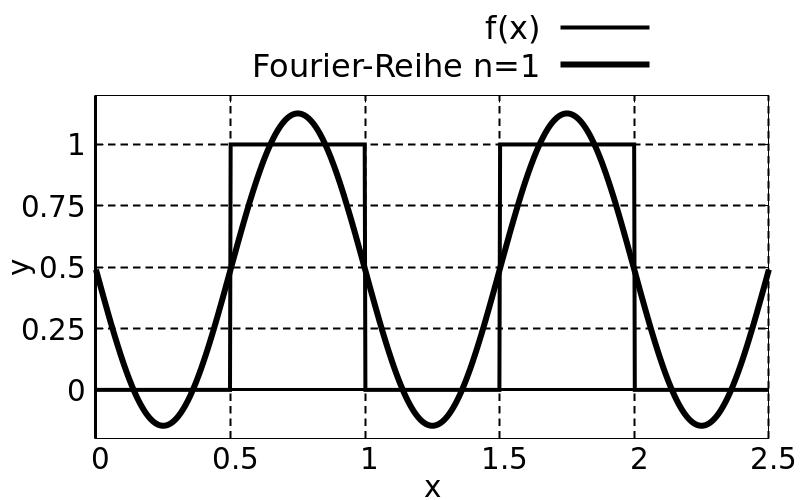
\includegraphics[width=0.45\textwidth]{./gnuplot/fourier-transform-step-1}
    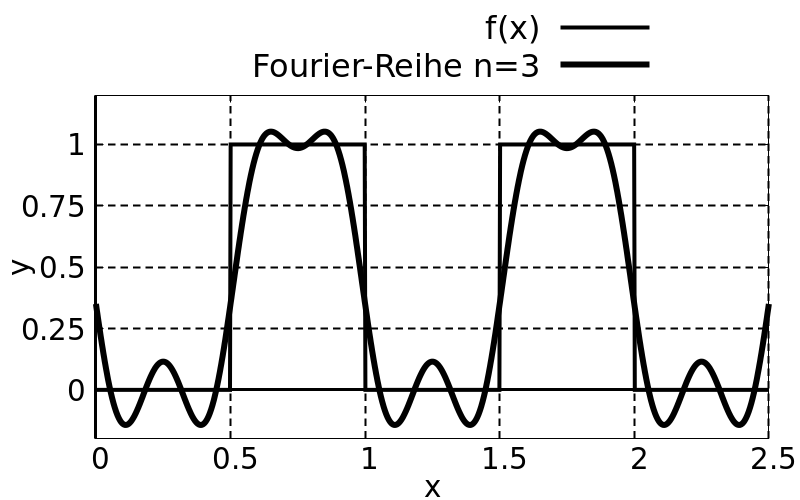
\includegraphics[width=0.45\textwidth]{./gnuplot/fourier-transform-step-2}
    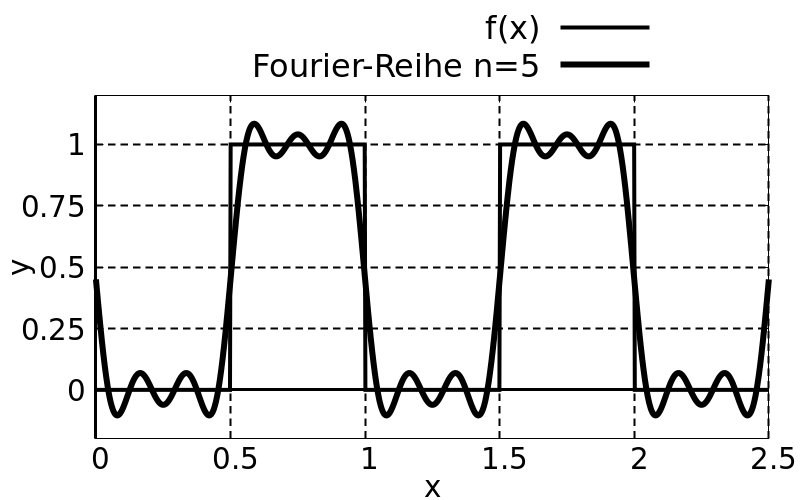
\includegraphics[width=0.45\textwidth]{./gnuplot/fourier-transform-step-3}
    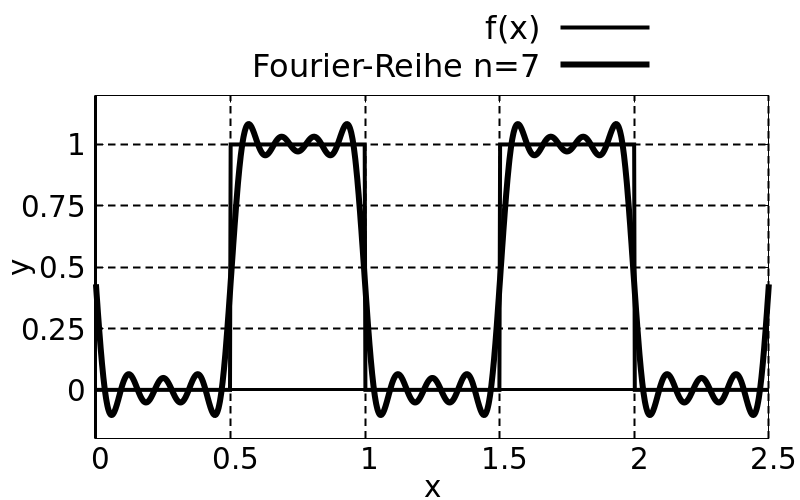
\includegraphics[width=0.45\textwidth]{./gnuplot/fourier-transform-step-4}
    \caption{Erste Glieder der Fourier-Rehe einer Einheitsschrittfunktion}
    \label{fig:ExUnitStepFourier}
\end{figure}

Nun ist es im Gegensatz zu Potenzreihen nicht so, dass die trigonometrische Reihe immer gleichmäßig konvergiert. Es gilt allerdings, dass wenn die Fourier-Reihe einer $f$ gleichmäßig konvergent ist, dass sie dann auch $f$ als Grenzfunktion hat, das Restglied also verschwindet. Diese Bedingung ist eine hinreichende, jedoch keine notwendige. Eine für die Praxis meist bessere Bedingung gibt der folgende Satz:

\begin{statement}{Dirichletsche Bedingung}{DirchCondFourier}
    Sei $f$ ein beschränkte, periodische Funktion mit der Periode $T$ und definiert im Intervall $[0,T)$. Wenn sich das Intervall $(0,2\pi)$ zerlegen lässt in endlich viele Teilintervalle, in derem jeden die Funktion $f$ stetig und monoton ist, so konvergiert die durch die Funktion $f$ erzeugte Fourier-Reihe für jede Stetigkeitsstelle $x_0$ gegen den Funktionswert $f(x_0)$ und für jede Sprungstelle $x_S$ gegen das arithmetische Mittel aus links- und rechtsseitigen Grenzwert $\frac{1}{2} \cdot \left(\lim\limits_{x\to x_S^-} + \lim\limits_{x\to x_S^+}\right)$.
\end{statement}

Das heißt also, dass wir im Gegensatz zur Taylor-Entwicklung mit der Fourier-Entwicklung auch unstetige Funktionen darstellen können. Beispielsweise werden in der Tontechnik und Elektrotechnik Rechteckimpulse verwendet, der dadurch gekennzeichnet ist, dass er innerhalb eines Intervalls den Wert $1$ und außerhalb davon den Wert $0$ besitzt. An der Grenze liegt also eine Sprungstelle vor. Dennoch kann man eine Fourier-Entwicklung durchführen und die Frequenzen des Rechteckimpulses ermitteln. In Abbildung \ref{fig:ExFourierDirichlet} ist dies am Beispiel einer Funktion mit mehreren Unstetigkeitsstellen dargestellt.

\begin{figure}
    \centering
    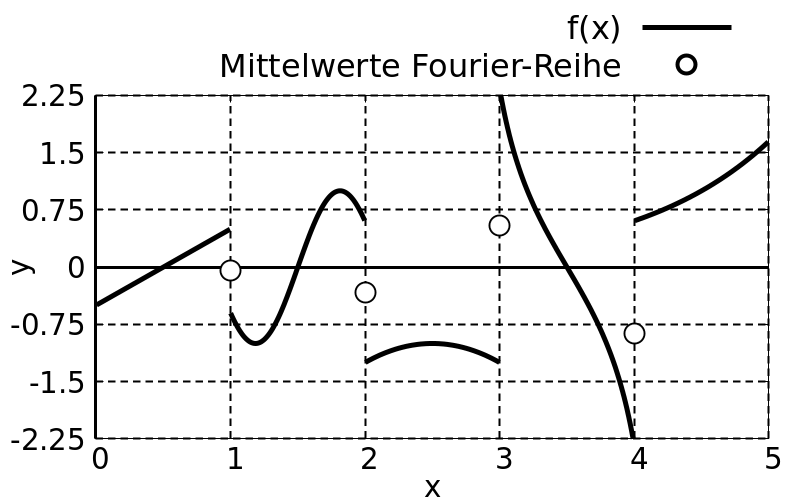
\includegraphics[width=0.65\textwidth]{./gnuplot/fourier-dirichlet}
    \caption[Fourier-Reihe einer unstetigen Funktion]{Unstetige Funktion und die Grenzfunktion der durch sie erzeugten Fourier-Reihe. Beide stimmen in allen Stetigkeitsstellen überein. An den Unstetigkeitsstellen wird das arithmetische Mittel zwischen links- und rechtsseitigen Grenzwert angenommen.}
    \label{fig:ExFourierDirichlet}
\end{figure}

\begin{example}{Grenzfunktion der Fourier-Reihe der Einheitsschrittfunktion}{ExUnitStepLim}
    Die Einheitsschrittfunktion aus Beispiel \ref{ex:ExFourUnitStep} lässt sich durch die Fourier-Reihe $\frac{1}{2} - \frac{2}{\pi} \sum\limits_{n=1}^\infty \frac{1}{2n-1} \sin(2\pi (2n-1) x)$ darstellen. Nun lässt sich die Einheitsschrittfunktion in die zwei Teilintervalle $(0, 0.5)$ und $(0,5, 1)$ zerlegen, in denen beiden sie stetig und monoton ist. Daher konvergiert sie dort gegen den Grenzfunktion, also die Einheitsschrittfunktion. Für $x=0,0.5,1.0,\dots$ konvergiert sich den Mittelwert aus links- und rechtssetigen Grenzwert, also gegen $\frac{1}{2} (0+1) = \frac{1}{2}$.
\end{example}

Zwei Bemerkungen noch zu praktischen Anwendungen. Zum einen können wir nicht nur eine Funktion auf ihre Frequenzen analysieren, sondern auch eine Funktion aus gegebenen Frequenzen zusammensetzen. Dies nennt man die sogenannten \emph{harmonische Synthese}. Diese wurde etwa früher genutzt, um gesprochene Sprache und Instrumententöne unter Anderem aus einfachen Sinus- und Kosinusschwingungen zusammenzusetzen. Da solche Signale aber komplexer sind, also aus mehr als einigen wenigen Frequenzen bestehen, lässt die Qualität dabei auch zu wünschen übrig. Daher werden heute meist aufgenommene Samples modifiziert und zusammengesetzt.

Zum Zweiten ist es so, dass man in der Praxis ein Signal nicht für jeden beliebigen Zeitpunkt kennt, um das Integral für die Koeffizienten der Fourier-Reihe bestimmten zu können. Aus dem Kapitel zur Infinitesimalrechnung wissen wir aber, dass das unbestimmte Integral als Grenzwert von Flächeninhaltssummen definiert war. Wenn wir das Signal beziehungsweise die Funktion nur an einer endlichen abzählbaren Menge von Stellen kennen, können wir die Fourierkoeffizienten mit einer endlichen Summenbildung statt dem Integral annähern.

\begin{definition}{Diskrete Fourier-Transformation}{DiscFourTrans}
    Eine Funktion $f$ mit der Periode $T$ sei im Intervall $[0, T]$ an den $2m$ Stellen $x_i = \frac{T}{2m} i$ ($0\le i < 2m-1$) gegeben mit den Funktionswerten $y_i$. Dann ist die die diskrete \textbf{Fourier-Transformation} definiert durch
    $$
        F[f](x) = a_0 + \sum\limits_{i=1}^m a_i \cos(\frac{2\pi}{T}ix) + b_i \sin(\frac{2\pi}{T}ix)
    $$
    Die Fourier-Koeffizienten berechnen sich dabei zu:
    \begin{alignat*}{1}
        a_0 &= \frac{1}{2m} \sum\limits_{i=0}^{2m-1} y_i  \\
        a_n &= \frac{1}{m} \sum\limits_{i=0}^{2m-1} y_i \cos(\frac{\pi}{m} ni) \\
        b_n &= \frac{1}{m} \sum\limits_{i=0}^{2m-1} y_i \sin(\frac{\pi}{m} ni) \\
        a_m &= \frac{1}{2m} \sum\limits_{i=0}^{2m-1} y_i \cos(i\pi)
    \end{alignat*}
\end{definition}

Ein Beispiel für das diskrete Frequenz-Spektrum eines Audio-Signals findet sich im Anhang in Abbildung \ref{fig:SpeechFreq}.

Bis hierher haben wir immer nur diskrete Frequenzen (Grundfrequenz $\frac{1}{T}$ und Vielfache) betrachtet. Abschließend sei noch angemerkt, dass es für einen kontinuierlichen Frequenz-Bereich noch die die sogenannte Fourier-Transformation gibt, welche einer Funktion ihre Fourier-Transformierte zuordnet:

$$
    \mathcal{F}[f(t)](\omega) = \frac{1}{\sqrt{2\pi}} \int\limits_{-\infty}^\infty f(t) e^{-j \omega t} \diff{t}
$$